\setchapterpreamble[u]{%
\dictum[René Descartes]{Vor eine Frage gestellt, die wir vollständig verstanden haben, müssen wir sie von jeder überflüssigen Darstellung abstrahieren, sie auf ihre einfachste Form reduzieren und sie in möglichst kleine Teile zerlegen, die wir dann aufzählen. \dots}}
\chapter{Analyse und Definition der Anforderungen } \index{Analyse und Definition der Anforderungen}\label{kap:analyse_und_definition}

Das \autoref{kap:aufgabenbeschreibung} erwähnt mehrere ISO Standards, welche zur Lösung der Problemstellung unterstützen können. In diesem Kapitel wird der ausgewählte ISO Standard ISO 29002-31 sowie der Standard ISO 22745-30 analysiert um festzustellen, wie und welche Anforderungen mit Hilfe dieser Standards umgesetzt werden können. 

Mittels den Erkenntnissen der Analyse werden Use Cases erarbeitet. 

\section{Analyse der ISO 29002-31 - Exchange of characteristics data}\label{kap:analyseiso2900231}\index{ISO 29002-31}

Ziel der Analyse ist es, herauszufinden ob die ISO-Norm zur Erfüllung der Anforderungen ausreichend ist, wie mit der ISO-Norm die Anforderungen umgesetzt werden können und ob gegebenenfalls weitere ISO-Normen zur Erfüllung der Anforderungen betrachtet werden müssen. 

Die gesamte Analyse der ISO 29002-31 mit Beschreibung der einzelnen Datencontainer findet sich in \autoref{kap:analyse2900231}. Die Analyse zeigt anhand von Beispielen auf, welche Abfragen mit der ISO 29002-31 möglich sind.

Zusammenfassend aus der Analyse ergeben sich folgende Abfragemöglichkeiten:
\begin{description}
\item[Simple Query] Eine Abfrage nach eindeutigem Identifier eines Konzeptes, mit der Möglichkeit der Einschränkung nach Eigenschaften eines Konzeptes (Projektion). Ferner ermöglicht der Simple Query die Übergabe bekannter Daten eines konkreten Teiles, nach denen gesucht und entsprechend passendes Ergebnis geliefert wird. Siehe dazu \autoref{sec:query}.
\item[Parametric Query] Ermöglicht die Abfrage nach eindeutigem Identifier eines Konzeptes und zusätzlich die Einschränkung einer Eigenschaft nach konkretem Wert (Selektion). Dies erfolgt mittels Angabe einer characteristic\_data\_query\_expression. Siehe dazu \autoref{sec:characteristicdataqueryexpression}.
\end{description}

Die konkreten Query Beispiele finden sich dazu in \autoref{kap:query_beispiele}.

\section{Analyse ISO 22745-30 - Identification Guide}\label{kap:identification_guide}\index{ISO 22745-30}

Ein Identification Guide beschreibt, welche Daten für ein Objekt benötigt werden, damit diese überhaupt sinnvoll für einen bestimmten Zweck eingesetzt werden können. Der Käufer, Produktmanager oder Benutzer definiert die Anforderungen an die Daten. Ein  \enquote{Datenanforderungsstatement} wird als ein i-xml, ein identification guide xml file, erzeugt. Siehe dazu auch \autoref{fig:lieferketten}. 

Es wird die Frage beantwortet, welche Daten und Eigenschaften zu einem bestimmten Konzept eines Objektes benötigt werden, um den Artikel beispielsweise zu kaufen oder sinnvoll zu verwalten. Diese Anforderungen werden von der Abfrageseite (Kundenseite) definiert, also diejenige, die Daten abfragen möchte \citep[Vergl.][]{bensonQuality}. 

Ein Identification Guide referenziert Konzepte eines Dictionaries um Datenanforderungen einer bestimmten Klasse zu beschreiben \citep[Vergl.][Kap. 5]{iso22745-30}.

Ein Datenempfänger kann eine Organisation oder eine Gruppe von Organisationen oder Firmen sein, welche ähnliche Datenanforderungen haben. Somit wird eine Identification Guide Gruppe von einer speziellen Organisation verwaltet, welche wiederum selbst Datenempfänger sein kann.  

Es kann somit festgehalten werden, dass für die Erfüllung der Aufgabenbeschreibung nach \autoref{kap:aufgabenbeschreibung} eine Implementierung des Standards ISO 22745-30 nicht notwendig ist, da dieser Standard eine zusätzliche Einschränkung der Konzepte und benötigten Daten auf Anfrageseite beschreibt. 
Die Abfrage gemäß einer SQL-Selektion und -Projektion ist mit dem Standard 29002-31 möglich. 

Basierend auf dieser Erkenntnis zeigt \autoref{fig:query_kombinationen} mögliche Abfrageinhalte und bewertet, ob diese umgesetzt werden müssen. Hierbei werden die Attribute \enquote{item\_description} und \enquote{data\_specification} nicht betrachtet.

\begin{figure}[htbp]
	\centering
		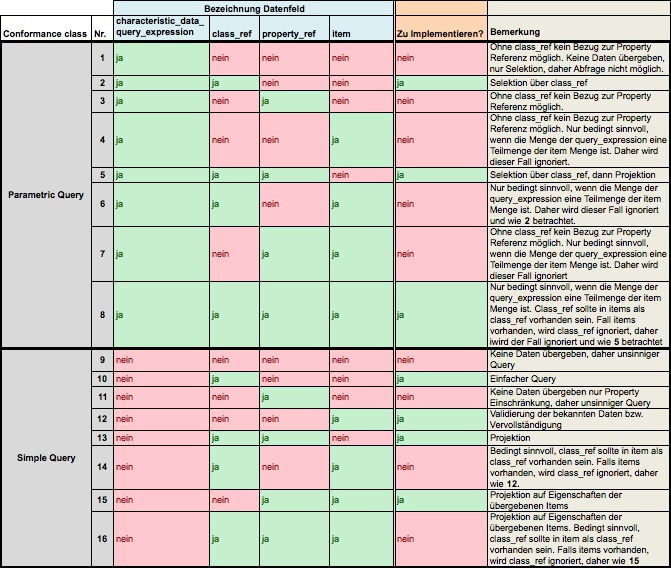
\includegraphics[width=0.90\textwidth]{images/queries.jpg}
	\caption{Mögliche Abfragen anhand der Kombination der Daten in XML Query}
	\label{fig:query_kombinationen}
\end{figure}

\section{Anwendungsfälle}\label{kap:Use_Cases}

Dieser Abschnitt beschreibt mögliche Anwendungsfälle\footnote{Use Case. Im weiteren Verlauf wird, gerade auch in den Anwendungsfallbeschreibungen von Use Cases gesprochen. Im deutschen Sprachraum ist das englische allgemein bekannte Äquivalent \enquote{Use Case} für Anwendungsfall eher geläufig als das deutsche, daher wird darauf verzichtet an manchen Stellen die Begrifflichkeiten einzudeutschen.} die sich aus ISO 29002-31 ergeben. 
Es wird beispielhaft ein Use Case aufgelistet und erläutert. Alle weiteren Use Cases sind in \autoref{kap:analyse_use_cases} zu finden. 

Die Query-Code-Beispiele sind gekürzt, d.h. es werden die referenzierte Schemata-Namen gemäß XSD nicht aufgeführt. 

\subsection{Was ist ein Use Case?}

Alistair Cockburn schreibt dazu \citep[Vergl.][Kap. 1.1]{cockburn2000}:

\begin{quotation}
\enquote{A use case captures a contract between the stakeholders of a system about its behavior. The use case describes the system’s behavior under various conditions as it responds to a request from one of the stakeholders, called the primary actor. The primary actor initiates an interaction with the system to accomplish some goal. The system responds, protecting the interests of all the stake- holders. Different sequences of behavior, or scenarios, can unfold, depending on the particular requests made and conditions surrounding the requests. The use case collects together those different scenarios.}
\end{quotation}

\gls{Stakeholder}\footnote{Stakeholder sind Projektbeteiligte, gleichsam Personen oder Institutionen und Dokumente, die in irgendeiner Weise vom Betrieb des Systems betroffen sind.} erwarten folglich ein gewisses Verhalten des Systems unter bestimmten Bedingungen. Dieses Verhalten des Systems in Interaktion mit Akteuren wird durch \glspl{Use Case} beschrieben.

\bild{usecases_plib.jpg}{13cm}{Use Case Übersicht}{Use Case Übersicht}

\subsection{Akteure}
Bei der Implementierung geht es um die Erstellung einer Software-Schnittstelle als \gls{Webservice}. Das bedeutet, dass diese Schnittstelle ohne eine Benutzeroberfläche nicht sinnvoll für einen menschlichen Akteur nutzbar ist. In den nachfolgenden Anwendungsfällen wird vom Akteur \enquote{Klient} gesprochen. Der Klient ist allgemein ein Nutzer der Schnittstelle, sei es als menschlicher Akteur welcher über eine Bedienerinterface die Schnittstelle benutzt oder eine direkte Maschinennutzung. Ein Beispiel für eine Maschinennutzung kann einen Anwendung sein, welche automatisiert die Schnittstelle aufruft und Daten abfragt.    

\subsection{Use Case Beschreibungen}

Da \glspl{Use Case} auf verschiedene Weise verfasst werden können, wird hier als Vorlage die \gls{Use Case} Beschreibungen aus dem Kurs Software Engineering I übernommen, da diese Vorlage sehr übersichtlich, knapp und präzise ist \citep[Vgl.][S. 120ff]{sixse1}. 

\subsubsection{Alle Charakteristische Daten eines Produkts abfragen}

{\small

\begin{description}
     \item[use case] Charakteristische Daten abfragen
     \item[  actors]~\\
     Klient
     \item[  precondition]~\\
     Der Klient verwendet einen gültigen Identifier.
     \item[  main flow]~\\
     Der Klient gibt einen eindeutigen Identifier (\gls{IRDI}\footnote{International Registration Data Identifier}) eines Konzeptes von Elementen ein und sendet eine Anfrage ab. Die Anfrage wird auf Gültigkeit überprüft. Als Antwort bekommt er ein oder mehrere Datensätze von Elementen\footnote{Item, ISO 29002-10 Kapitel 5.3.2} mit den entsprechenden charakteristischen Daten\footnote{property\_values, ISO 29002-10 Kapitel 5.2.4}  des Elementes mit dem übergebenen Identifier zurück.
     \item[  postcondition]~\\
     Alle Daten aller Elemente der gewählten Konzepte des Identifiers wurden zurückgegeben.    
     \item[  alternative flow] Properties auswählen ~\\
     Zusammen mit dem Identifier übergibt der Klient einen oder mehrere Property-Identifier und sendet diese erweiterte Anfrage ab.    
     \item[  postcondition]~\\
     Die mittels Property-Identifier ausgewählten Daten aller Elemente der gewählten Konzepte wurden zurückgegeben.    
     \item[end] Charakteristische Daten abfragen
\end{description}

~\\

} %end small

\subsubsection{Beispiel}\label{lab:schraubendreher}

Ein Schraubendreher könnte folgendermaßen in einer Produktdatenbank repräsentiert werden:

\begin{description}
\item[Klassen-Identifier] 0173-1\#01-AAA352\#4 
\item[Länge] 300mm
\item[Typ] Kreuz
\item[Spannungsfest] ja
\end{description}

Korrekterweise müssten anstatt der Attribute wie Länge oder Typ ebenfalls ein Identifier stehen. Die Benamungen sind hier zur besseren Lesbarkeit aufgelöst. 

Um alle Eigenschaften (Properties) wie Länge, Typ und Spannungsfest zu erhalten, muss folgende Abfrage gesendet werden: 
\begin{quotation}
\enquote{Gib mir alle \glslink{item}{Teile} und alle Properties der Klasse mit dem Identifier 0173-1\#01-AAA352\#4 (Schraubendreher).}
\end{quotation}

Das Ergebnis ist ein \gls{item} mit allen Attributen (Properties) der gewünschten Konzepte und gegebenenfalls vorhandenen Unterkonzepte. In unserem Falle genau die oben angegebenen Werte.

Die XML-Abfrage sieht wie folgt aus:

\begin{lstlisting}[caption=Query Beispiel - alle Daten abfragen, language=XML, label=UseCaseDatenabfragen]
<?xml version="1.0" encoding="UTF-8"?>
<qy:query xsi:schemaLocation="...query query.xsd" xmlns:xsi="http://www.w3.org/2001/XMLSchema-instance" xmlns:cat="...catalogue" xmlns:val="...value" xmlns:qy="...query" xmlns:bas="...basic">
	<qy:class_ref>0173-1#01-AAA352#4</qy:class_ref>
</qy:query>
\end{lstlisting}

Eine Abfrage, welche als Projektion die Properties der Klasse auswählt, die zurückgeliefert werden sollen, könnte lauten: 
\begin{quotation}
\enquote{Gib mir alle \glslink{item}{Teile} und die Properties Länge und Typ der Klasse mit dem Identifier 0173-1\#01-AAA352\#4 (Schraubendreher).}
\end{quotation}

Das Ergebnis ist ein \gls{item} mit den gewünschten Attributen (Properties). 

Die XML-Abfrage lautet:
\begin{lstlisting}[caption=Query Beispiel - Daten abfragen mit Propertyeinschränkung (Projektion), language=XML, label=lst:UseCaseDatenabfragenProperty]

<?xml version="1.0" encoding="UTF-8"?>
<qy:query xsi:schemaLocation="...query query.xsd" xmlns:xsi="http://www.w3.org/2001/XMLSchema-instance" xmlns:cat="...catalogue" xmlns:val="...value" xmlns:qy="...query" xmlns:bas="...basic">
	<qy:class_ref>0173-1#01-AAA352#4</qy:class_ref>
	
	<!-- identifier von typ und laenge werden uebergeben -->
	<qy:property_ref>0173-1#01-BBB111#1 0173-1#01-BBB222#1</qy:property_ref> 
	
</qy:query>
\end{lstlisting}

\autoref{lst:UseCaseDatenabfragenProperty} beinhaltet ein XML-Attribut property\_ref. Das wird mit gewünschten Property Identifier gefüllt, welche mit Leerzeichen getrennt werden. 


\section{Zusammenfassung des Kapitels}

Das Ergebnis der Analyse der Standards ISO 29002-31 und 22745-30 ergibt, dass diese Beschreibungen für die Lösung der Problemstellung, die Entwicklung einer \gls{Abfrageschnittstelle} analog zur SQL-Selektion und -Projektion der Standard ISO 29002-31, ausreichend sind. Sowohl Projektion als auch Selektion ist dadurch möglich. ISO 22745-30 beschreibt als \gls{IG} eine weitere klientseitige Einschränkung der abzufragenden Daten. Man stelle sich eine Einschränkung (Definition einer Teilmenge) durch ein Formular vor. Das Formular schränkt die abzufragenden Daten auf die tatsächlich benötigte Menge von Daten gegebenenfalls stark ein und gibt ebenfalls den Typ der Daten vor. Dies wird durch Referenzieren auf Konzepte eines Dictionaries erreicht.

Aus den Anforderungen wurden sinnvolle \glspl{Use Case} formuliert, welche das Verhalten des Systems beschreiben sollen.  
